\documentclass{article} % For LaTeX2e
\usepackage{nips15submit_e,times}
\usepackage{url}
\usepackage[pdftex]{graphicx}
\usepackage{fullpage}
\usepackage{listings}
\usepackage{amssymb}
\usepackage{cite}
\usepackage{amssymb,amsfonts,amsmath,amscd}
\usepackage[pdftex,colorlinks]{hyperref}
\usepackage{fnpos}
\usepackage{subfigure}
\usepackage{verbatim}
\usepackage{fancyhdr}
\usepackage{pifont}


% Some handy commands
\newcommand{\norm}[1]{\left\Vert#1\right\Vert}
\newcommand{\abs}[1]{\left\vert#1\right\vert}
\newcommand{\set}[1]{\left\{#1\right\}}
\newcommand{\Real}{\mathbb R}
\newcommand{\Complex}{\mathbb C}
\newcommand{\eps}{\varepsilon}
\newcommand{\To}{\longrightarrow}
\newcommand{\Ker}{\textup{Ker}}
\newcommand{\Img}{\textup{Img}}
\newcommand{\diag}{\textup{diag}}
\newcommand{\circulant}{\textup{circ}}
\newcommand{\bs}[1]{\boldsymbol{#1}}

% checks and Xs
\newcommand{\yes}{\ding{51}}
\newcommand{\no}{\ding{55}}

% Tim's Math Defs
\newcommand{\bcf}{\;\mbox{\boldmath ${\cal F}$\unboldmath}}
\def\Vec#1{\!\!\hbox{$#1$\kern-0.38em\lower0.85em\hbox{$\vec{}\,$}}\,}%
\newcommand{\bbm}{\begin{bmatrix}}
\newcommand{\ebm}{\end{bmatrix}}
\DeclareMathAlphabet{\mbf}{OT1}{ptm}{b}{n}
\newcommand{\mbs}[1]{{\boldsymbol{#1}}}
\def\ep{\epsilon}
\def\la{\lambda}
\def\om{\omega}
\newcommand{\qc}[1]{{#1}^+}
\newcommand{\qo}[1]{{#1}^\oplus}
\newcommand{\qi}[1]{{#1}^{\scalebox{0.5}{$-1$}}}

% Math Defs
\def\N{\ensuremath{\mathcal{N}}}
\newcommand{\normpdf}[2]{\mathcal{N}(#1|\mu_#2,\sigma_#2^2)}
\newcommand{\gaussian}[2]{\frac{1}{\sigma_#2\sqrt{2\pi}}e^{-\frac{(#1-\mu_#2)^2}{2\sigma_#2^2}}}
\newcommand{\pd}[2]{\frac{\partial #1}{\partial #2}}
\newcommand{\ds}{\displaystyle}

\nipsfinalcopy{\nipsfinaltrue}

\title{The Superpixel Superhighway: A Comparison of Machine Learning Algorithms for Road Classification}

\author{
Jacob Lambert\\
Institute for Aerospace Studies\\
University of Toronto\\
\texttt{jacob.lambert@mail.utoronto.ca} \\
\And
Rikky Duivenvoorden\\
Institute for Aerospace Studies\\
University of Toronto\\
\texttt{rikky.duivenvoorden@mail.utoronto.ca} \\
}

\begin{document}

\maketitle

\begin{abstract}
In this paper, we show how to solve robotics using machine learning.
\end{abstract}

\section{Introduction}

\subsection{Related Work}

\section{Dataset}
\subsection{KITTI}
The dataset used in these experiments is provided by the Karlsruhe Institute of Technology (KIT) and Toyota Technological Institute (TTI) in Chicago[1]. This vision benchmarking suite has become a standard for comparing the performance of algorithms for tracking, navigation, estimating scene flow and object segmentation and classification.

The dataset for road classification is seperated in three different environments: urban unmarked (uu), urban marked (um) and urban multiple marked lanes (umm), each shown in figure \ref{fig:kitti}. Each set contains roughly a hundred RGB images of size $375\times1242$ pixels, taken from a monocular camera mounted on top of a car.

\begin{figure}[ht!]
\centering
 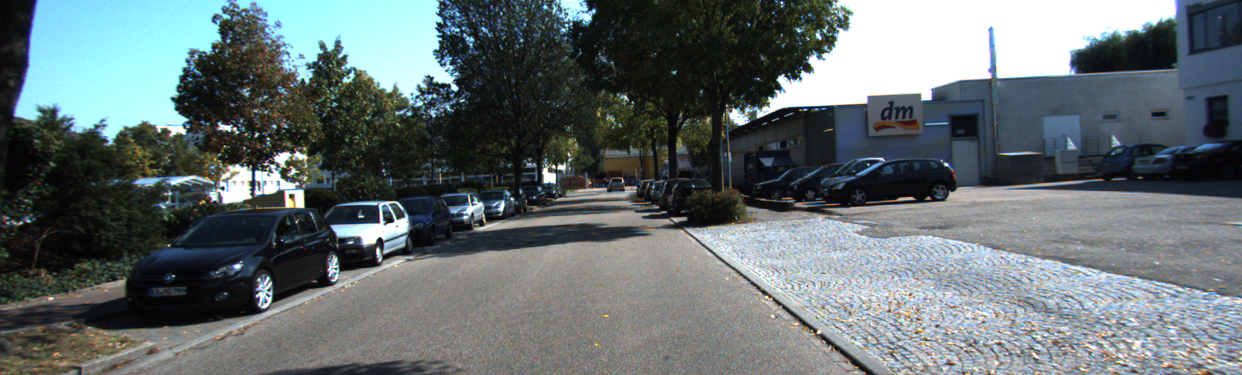
\includegraphics[width=0.3333\linewidth]{figs/uu_example.png}\hspace{-3pt}
 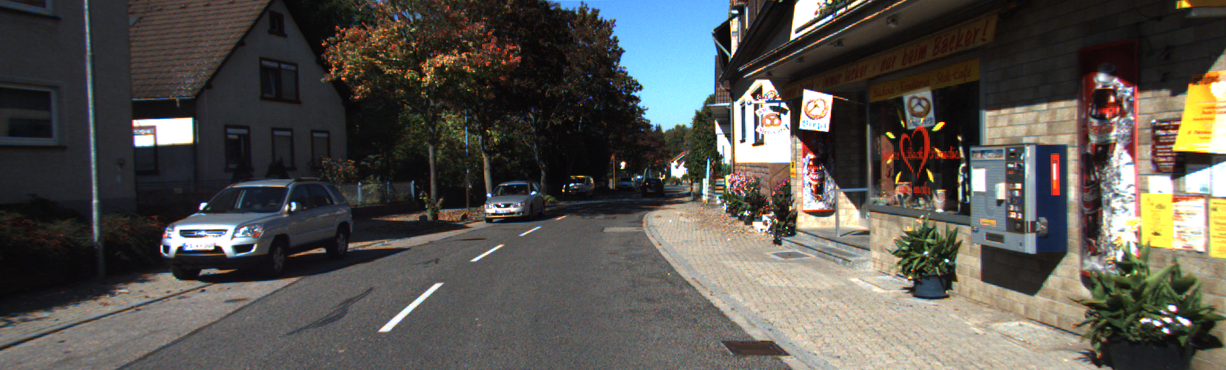
\includegraphics[width=0.3333\linewidth]{figs/um_example.png}\hspace{-3pt}
 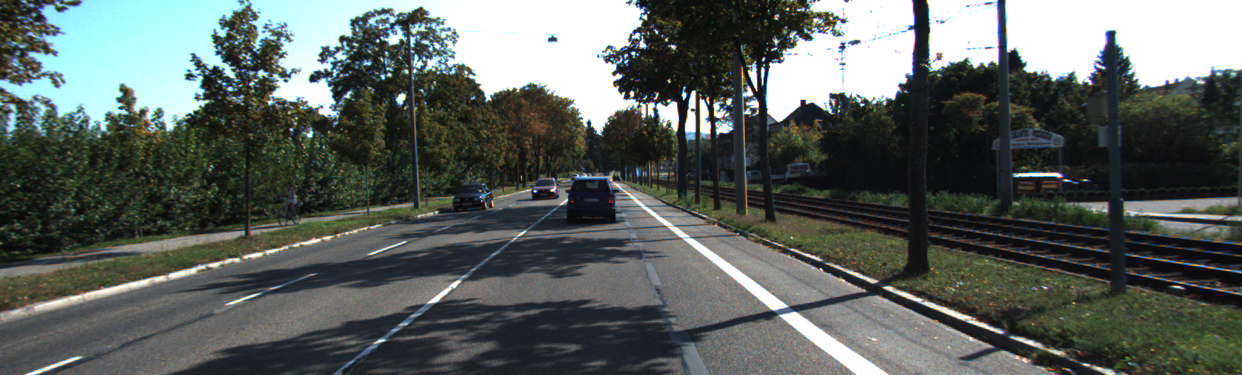
\includegraphics[width=0.3333\linewidth]{figs/umm_example.png}
\caption{The three environments in the KITTI dataset: uu (left), um (middle) and umm (right)}\label{fig:kitti}
\end{figure}

The urban unmarked environment is the most challenging of the three as the typical images are of narrow roads in dense city environments. There are several obstructions, some static such as shadows, parked vehicles or street signs, and others dynamic like pedestrians, cyclists and moving vehicles. There are also several intersection parking lots or driveways which are visually very similar to roads, but they are not included in the ground truth image. Figure \ref{fig:gt} shows the ground truth image for the left most image in figure \ref{fig:kitti}. The urban marked dataset features similar scenes but with road markers, delimiting lanes and often the side of the road, making the segmentation and classification task slightly easier. urban multiple marked lanes contains images of larger roads such as boulevards or highways. The scenes in this dataset are typically much less cluttered than the former two and the roads have clear delimiters.

\begin{figure}[ht!]
 \centering
 
\includegraphics[width=0.5\textwidth]{figs/gt_example_uu.png}
 \caption{Ground truth image for the left-most image in figure \ref{fig:kitti} provided in the KITTI dataset. Pink pixels are classified as road and red pixels as non-road.}\label{fig:gt}
\end{figure}

\subsection{Superpixel Segmentation}
While the classification could be performed for each pixel, the approach taken in this work is to first segment each image into a set of superpixels. There are several advantages to this, the first and foremost is that it heavily reduces training time; there are approximately 46 million pixels per dataset. If we can segment the image into a set of similar looking patches, we heavily reduce the number of training examples without losing much information. Furthermore, the information provided by individual pixels is limited by the RGB color intensities and the pixel position. A set of pixels allows us to compute a variety of features, as dicussed in section \ref{sec:feat}. Superpixel segmentation essentially allows us reduce the number of examples while increasing the dimensionality of each examples.

Here we use the Simple Linear Iterative Clustering (SLIC) algorithm[2] to segment the each image in approximately $750$ superpixels. The algorithm creates superpixels by clustering pixels of similar colors. Intuitively, the approach is adequate for segmenting roads as we expect them to be uniform in color but figure \ref{fig:SLIC} shows that SLIC performs poorly in a variety of scenarios. Notable examples are driveways which SLICO fails to segment in the top image  of figure \ref{fig:SLIC}. In the middle image, SLIC manages to segment the road from the grassy region on the left, but fails to properly differentiate road from sidewalk on the right. In the bottom image, SLIC segments all shadows in the scene regardless of the actual scene content. The images in each respective datasets are similar and as such there were many cases of poor segmentation which inevitably led to several superpixels representing both road and not-road. Classification on those superpixels is especially challenging, as shown in section \ref{sec:results}

\begin{figure}[ht!]
\centering \hspace{-1.1pt}
 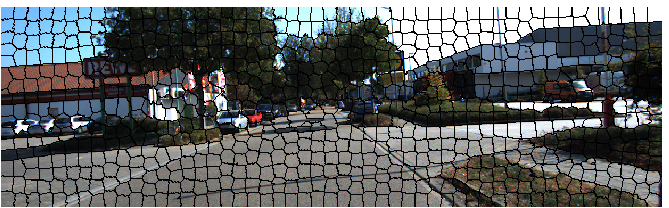
\includegraphics[width=0.5045\textwidth]{figs/SLICOuu.pdf}\\
 \vspace{-2.2pt}
 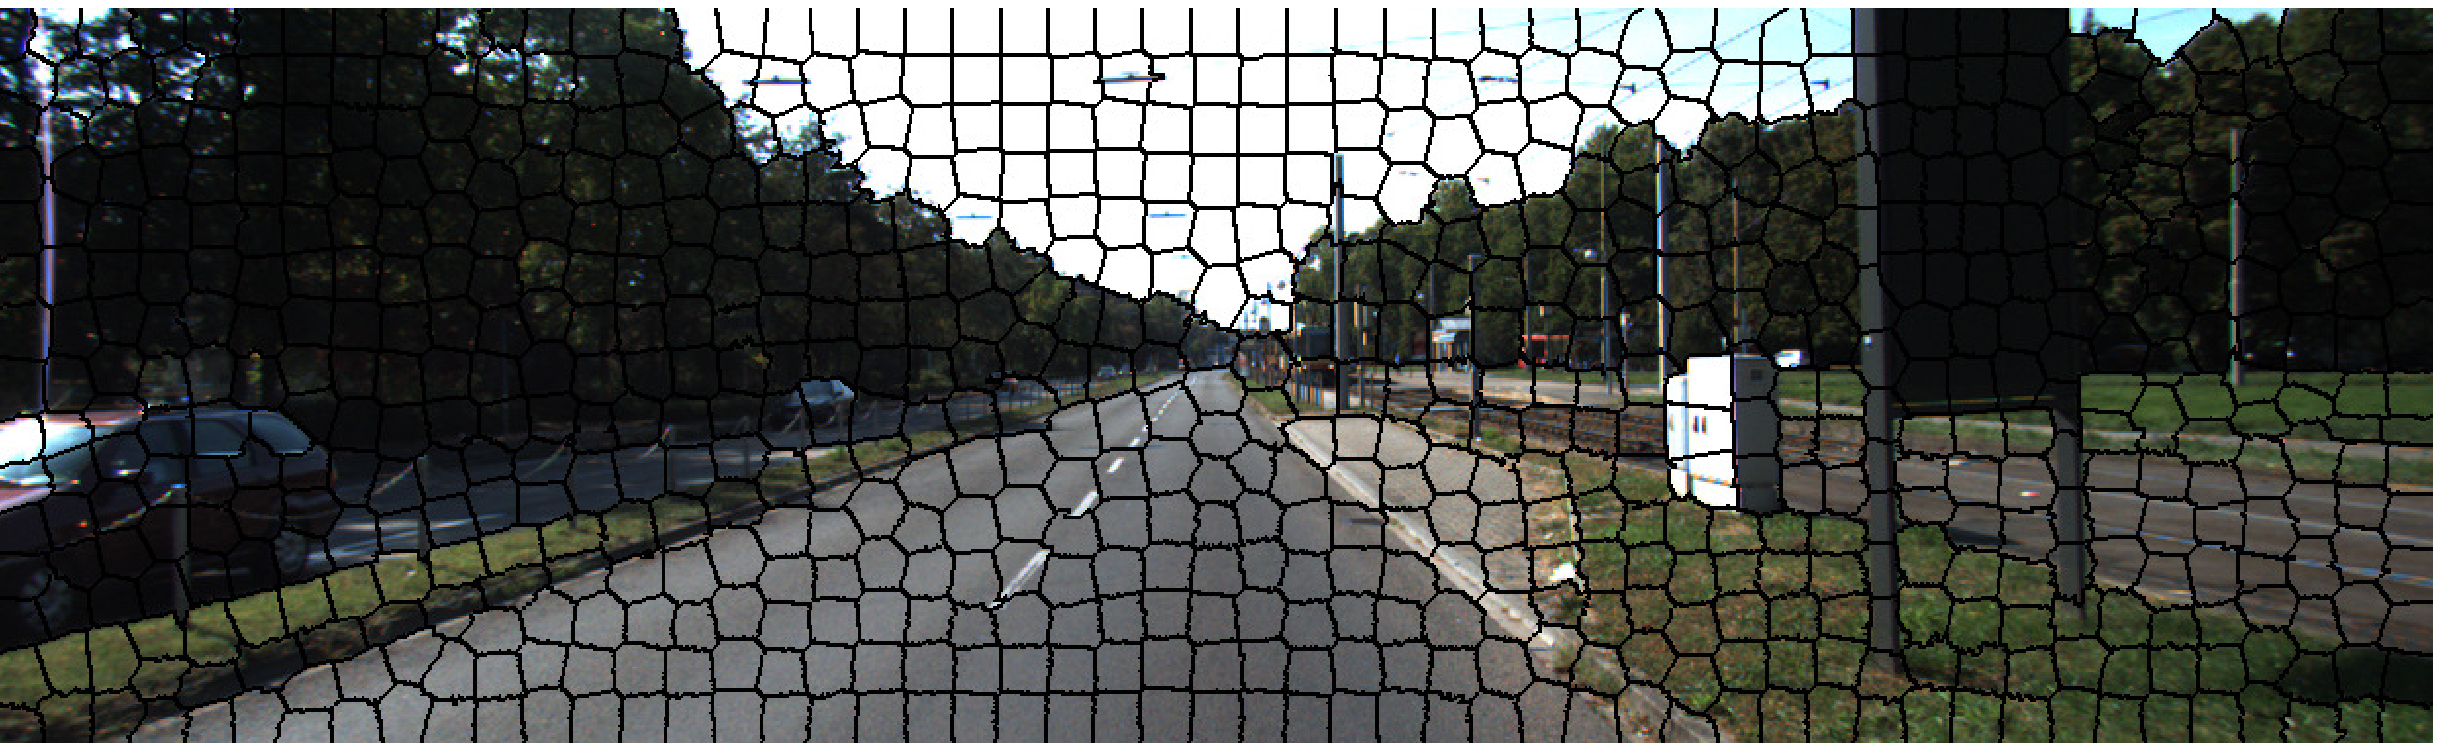
\includegraphics[width=0.5\textwidth]{figs/SLICOum.pdf}\\
 \vspace{-4.0pt} \hspace{-1.1pt}
 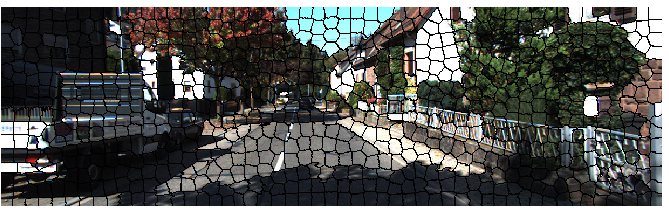
\includegraphics[width=0.5045\textwidth]{figs/SLICOumm.pdf}\\
 \caption{Performance of the SLIC algorithm on the uu dataset (top), um dataset (middle) and umm dataset .}\label{fig:SLIC}
\end{figure}

As the segmentation is imperfect, some superpixels will inevitably contain positive and negative examples. To solve this issue, a new ground truth image was created (shown in figure \ref{fig:SLICgt}), where each superpixel was classified based on the majority of pixels in its cluster.

\begin{figure}
 \centering
  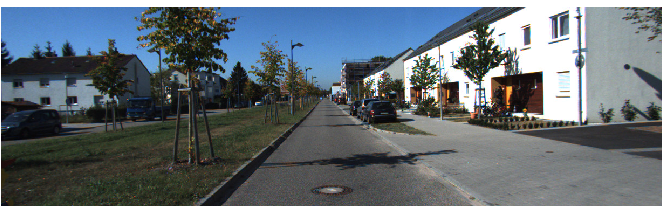
\includegraphics[width=0.49\linewidth]{figs/noSLICimage.pdf}\hspace{-3pt}
  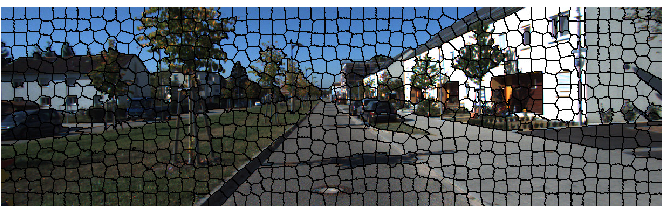
\includegraphics[width=0.49\linewidth]{figs/SLICimage.pdf}\hspace{-3pt}\\
  \vspace{-2pt}
  
\includegraphics[width=0.49\linewidth]{figs/noSLICgt.pdf}\hspace{-3pt}
  
\includegraphics[width=0.49\linewidth]{figs/SLICgt.pdf}
  \caption{The image segmentation pipeline is shown here. The starting image (top left) is first segmented into superpixels by SLIC (top right) then the label (bottom left) is adjusted to be uniform within superpixels (bottom right).}
\end{figure}


\subsection{Feature Selection}\label{sec:feat}

The types of feature computed for each superpixel is a critical step in the classification pipeline as they need to convey enough information about the superpixel to allow classification. In this experiment chose a total of 14 simple and intuitive features. An example $\mbf{x}^{(i)}$ is stored as

\begin{equation}
 \mbf{x}^{(i)} = 
 \begin{bmatrix}\mbf{r}^{(i)}~~\bs{\mu}_{RGB}^{(i)}~~\bs{\sigma}_{RGB}^{(i)}~~\bs{\mu}_{\nabla RGB}^{(i)}~~\bs{\sigma}_{\nabla RGB}^{(i)}  \end{bmatrix}.
\end{equation}
$\mbf{r}^{(i)}=\left[x^{(i)}~~ y^{(i)}\right]$ is the centroid of the superpixel. For the $i$th superpixel composed of N pixels each with location $\mbf{r}^{(i)}_n$, the centroid is given by
\begin{equation}
 \mbf{r}^{(i)} = \frac{1}{N}\sum_{n=1}^N \mbf{r}^{(i)}_n.
\end{equation}

Then, $\bs{\mu}_{RGB}^{(i)} = \left[\mu_{R}^{(i)}~~\mu_{G}^{(i)} ~~\mu_{B}^{(i)}  \right]$ and $\bs{\sigma}_{RGB}^{(i)} = \left[\sigma_{R}^{(i)}~~\sigma_{G}^{(i)} ~~\sigma_{B}^{(i)}  \right]$ are the respective pixel intensity mean and variance for Red, Blue and Green color channels. Finally, we compute the gradient magnitude of the image in each color channel, which produces an image shown in figure \ref{fig:grad}. As computing the gradient picks out high frequency color variations, we expect it to pick out edges or high irregular regions like vegetation. Roads which are uniform should have low gradient magnitude and even lower variation. $\bs{\mu}_{\nabla RGB}^{(i)}$ and $\bs{\sigma}_{\nabla RGB}^{(i)}$ are then the mean color and variation for each color channel in the gradient image.

\begin{figure}[ht!]
\centering
 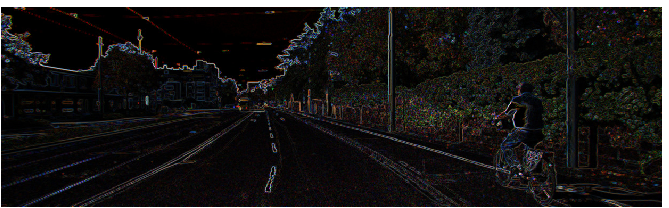
\includegraphics[width=0.7\textwidth]{figs/grad.pdf}\\
 \caption{Gradient magnitude of one of the images.}\label{fig:grad}
\end{figure}



\section{Algorithms}
\subsection{\textit{k} Nearest Neighbors}
\subsection{Support Vector Machines}

Initial testing of SVMs revealed that their ability to generalize depended heavily on the size of the dataset. As using 70\% of the dataset for training led to comparitively poor results, we tested several kernels for various fractions of the dataset as shown in table \ref{tab:svm}

\begin{table}[ht!]
 \begin{tabular}{c | c 
  
 \end{tabular}
\end{table}


\subsection{Neural Network}

\section{Results}\label{sec:results}

\section{Discussion}

\subsubsection*{References}

% \small{
% [1] Alexander, J.A. \& Mozer, M.C. (1995) Template-based algorithms
% for connectionist rule extraction. In G. Tesauro, D. S. Touretzky
% and T.K. Leen (eds.), {\it Advances in Neural Information Processing
% Systems 7}, pp. 609-616. Cambridge, MA: MIT Press.
% 
% [2] Bower, J.M. \& Beeman, D. (1995) {\it The Book of GENESIS: Exploring
% Realistic Neural Models with the GEneral NEural SImulation System.}
% New York: TELOS/Springer-Verlag.
% 
% [3] Hasselmo, M.E., Schnell, E. \& Barkai, E. (1995) Dynamics of learning
% and recall at excitatory recurrent synapses and cholinergic modulation
% in rat hippocampal region CA3. {\it Journal of Neuroscience}
% {\bf 15}(7):5249-5262.
% }
\small{
[1] A. Geiger, P. Lenz \& R. Urtason, (2012) Are we ready for Autonomous Driving? The KITTI Vision Benchmark Suite. {\it Conference on Computer Vision and Pattern Recognition (CVPR)}, Providence, RI.

[2] R. Achanta, A. Shaji, K. Smith, A. Lucchi, P. Fua, \& S. Süsstrunk, (2012) SLIC Superpixels Compared to State-of-the-art Superpixel Methods. {\it IEEE Transactions on Pattern Analysis and Machine Intelligence}, {\bf 34}(11):2274-2282.

}

\end{document}
